
\documentclass[a4paper,12pt,leqno]{article}%{tudscrreprt}% leqno left equation numbering
%\documentclass[a4paper,12pt]{article}%{tudscrreprt}%
\def\dotminus{\mathbin{\ooalign{\hss\raise1ex\hbox{.}\hss\cr
			\mathsurround=0pt$-$}}
		}
\usepackage[a4paper,margin=2cm]{geometry}	% margins and paper set
\usepackage{hyperref}
\usepackage{xcolor}
\usepackage{graphicx}
% % % some math packs
\usepackage{amsmath,amssymb,amsfonts,amsthm}
\usepackage{mathtools}
\usepackage{ntheorem}
%\usepackage{package}
%opening
% % enviroments without numering
\newtheoremstyle{plain}%    <name>
{\topsep}%   <space above>
{\topsep}%   <space below>
{\upshape}%  <body font>
{}%          <indent amount>
{\bfseries}% <Theorem head font>
{.}%         <punctuation after theorem head>
{\newline}%  <space after theorem head> (default .5em)
{}%          <Theorem head spec>
\theoremstyle{plain}
\newtheorem*{example}{Example}

% % % comamnds % % %
\newcommand{\ul}[1]{\underline{#1}}
\renewcommand{\emph}[1]{\textit{#1}}
\newcommand{\important}[1]{\textbf{#1}}
%notes
\newcommand{\notes}[1]{\textcolor{red}{#1}}
\newcommand{\todo}[1]{\textcolor{blue}{#1}}
\newcommand{\idea}[1]{\textcolor{green}{#1}}
% text stuff in math
\newcommand{\odd}{\text{odd}}
\newcommand{\even}{\text{even}}
\newcommand{\for}{\text{ for }}
\newcommand{\with}{\text{ with }}
\newcommand{\const}{\text{ const. }}

\title{Tips and Tricks for WALDORF MicroWave II and the XT Version}
\author{Ameyah and Various}

\begin{document}

\maketitle
\begin{abstract}
	\noindent
	This is a collection notes from various authors on tips and tricks for the Microwave II, so that its possible to quickly print them or have them available for browsing. The author of this document is thankful to the other authors of the quotes here.\\
	\today
\end{abstract}

\newpage

\tableofcontents

\newpage

\section{Introduction}
% !TeX spellcheck = en_US
This little quick tour from here: \href{https://www.carbon111.com/xt_intro.html}{Carbon111}
\subsection{A Quick Tour of the MicrowaveII/XT}
If you need a quick introduction to the Microwave II/XT or just want to know what all the fuss is about, here you go.
Welcome to my quick tour of the Microwave II/XT/XTk (for simplicity's sake hereafter refered to as the XT). If you are familiar with Subtractive Analog synthesis then you will readily understand the XT. First, lets look at a block diagram of how the WaveXT is laid out - this will be our "roadmap":
A complete answer for just reference.
\bigskip % Add an empty line
%These are optional parameters to finetune the placement of tables and figures, with the following meaning:
%
%h, here
%t, top
%b, bottom
%p, page of float
%e.g. \begin{figure}[!htb]
\begin{figure}[ht!]
	\centering
	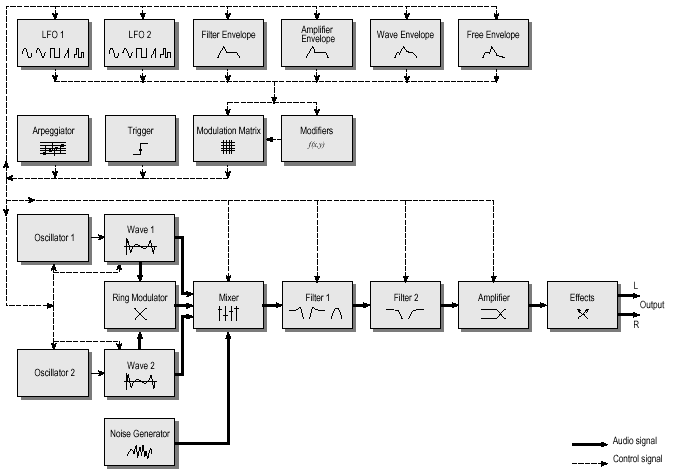
\includegraphics[width=90mm]{pics/mwxt_block.png}
	\caption{Microwave II block diagram}
	\label{blockdiagrammwxt}
\end{figure}
\paragraph{Oscillators and Wavetables}
Our First stop is the Oscillators. The XT has two of these. Unlike a standard analog synthesizer, the oscillators aren't heard directly - they merely drive the frequency of the waveform generators for the currently chosen wavetable. If this doesn't make sense immediately, don't worry about it, just remember that the oscillators drive the pitch of the currently chosen wavetable wave. The oscillators and wavetabes (and, for that matter, even the filters) of this synth make no apologies about being unabashedly digital.\\
Wavetable synthesis is characterized by the ability to sequence through a table of different waveforms during the duration of a single note. The XT has 65 preset wavetables and 32 user-programmable wavetables. A wavetable can be pictured as a row of 64 pointers to any of the 300 waveforms stored in the XT's ROM memory or any waveforms available in the user memory. Lets look at wavetable 016 "Square Saw" as an example:
\begin{figure}[ht!]
	\centering
	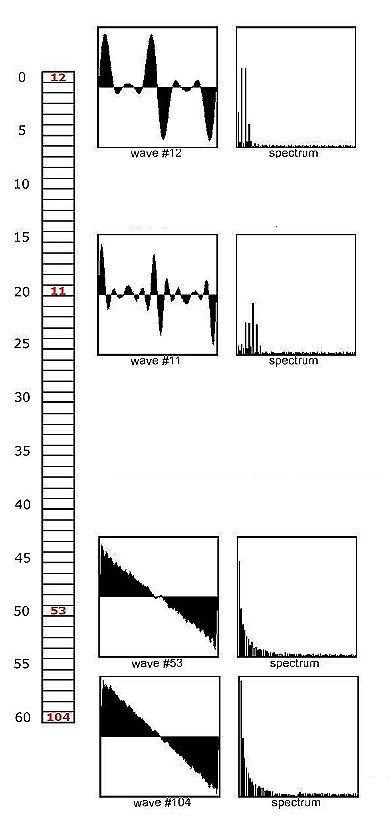
\includegraphics[width=90mm]{pics/osc_wt.jpg}
	\caption{pointers and wavetable with spectrum}
	\label{osc_wt}
\end{figure}
At position 0 is a pointer to ROM waveform \#12, a waveform with strong 2nd and 3rd harmonics, vaguely reminiscent of a square wave. The next pointer is at position 20 for ROM wave \#11, similar to \#12 but with higher harmonics. Next at position 50 is ROM wave \#53, very close to a sawtooth wave. Finally at position 60 is ROM wave \#104, a familiar classic ``buzzy'' sawtooth. The table positions from 1 - 19, 21 - 49 and 51 - 59 are interpolated by the XT automatically. If you move the start wave up or down the wavetable with an envelope, LFO or even the modwheel, you get a smooth transition between each of the four ``real'' waveforms because of the crossfading or "morphing" caused by the XT's interpolation to fill in the gaps.\\
So, if you were to set up a simple sound with just one oscillator with an initial start wave setting of 0 and a basic ramp envelope controlling wavetable position, when you struck a key, you would get a smooth sweep from a ``squarish-sounding'' wave \#12 all the way to a bright "buzzy" sawtooth wave \#103 without any gaps or glitches in between. Of course we are not limited to gentle sweeps with simple ramp EGs - we can use the powerful 8-time 8-level wave envelope generator with its sustain and release loops to create unique and complex timbral morphs if we want - and we do want!\\
The last three positions in each wavetable (61, 62 \& 63) are always reserved for the classic analog subtractive synth waveforms: saw, square and triangle so they are always available if needed. We can turn on a ``limit'' function for the oscillators so we don't unintentionally stray onto the analog waves when scanning the wavetable - a handy feature to avoid timbral glitches. Some of the wavetables in the XT emulate different types of filter sweeps, others offer simulated pulse width modulation, formant sweeps and other timbral morphs. These are designed to be swept with an envelope, LFO or smooth modulator of your choice. Other wavetables like 064 ``Chorus2'' are designed instead to make use of the keytrack parameter to keep a homophonic timbre across a number of octaves - changing the waveform depending on the key played. Still, other wavetables, like the four ``Wavetrip'' tables, are diverse collections of disparate waves well suited to creative cacophony and euphony of all kinds.\\
Hardwired to the wave position parameter of waveform generators 1 and 2 is the so-called wave envelope which is a very powerful 8-time 8-level complex envelope with user-adjustable looping points in the sustain and release segments. This envelope can be used to modulate other elements in the XT too through the modmatrix - more on that later.\\
Ring modulation, hard sync and glide are available for even more oscillator mayhem but lest we dwell too long at the start of our trip we forge on...
\paragraph{Filters}
Next on our journey are the filters. The XT is outfitted with two filters set up in series. The second filter is a basic 6dB filter switchable between lowpass or highpass - mainly used to ``tidy up'' the output of the first filter. The main filter on the XT is an amazing multimode beast with 10 different filter types - lets look at some of the more interesting possibilities:
\begin{itemize}
	\item 24dB and 12dB Lowpass: These are the ``classic'' analog-style filters used for most subtractive synthesis. The 24dB gives an ``aggressive'' filtered sound reminiscent of a Moog ``ladder'' while the 12dB offers a much softer slope much like the old Oberheim synths. Even though the XT is no ``virtual analog'', the filters can be very convincing depending on the application. 
	\item Sine Waveshaper and 12dB Lowpass: This filter packs a real punch with a tight compression sound provided by the sine waveshaper. Excellent on bass sounds.
	\item Waveshaper: This filter has some real suprises, similar to the Sine Waveshaper but with the ability to use any wave in the current wavetable as the shaper wave! Used with a square wave, this filter will rip your face off.
	\item Dual Lowpass/Bandpass: This is a dual filter combining a 12dB lowpass with a 12dB bandpass in series. Sweep different cutoff settings for each filter from different modulators to get amazing shimmering, ``swirling-in-front-of-your-face'' type sounds.
	\item S/H (Sample \& Hold) into 12dB Lowpass: This filter is a brutal sample-rate reduction processor combined with a standard 12dB lowpass. Make the XT sound like a really crappy, cheap low-res sampler! This is a good thing!
	\item There are six other filters as well but I will let you discover those for yourself.
\end{itemize}
Hardwired to the Filter is a basic ADSR envelope that can be used with or overridden by any modulation you choose. Modulating decay time with key velocity is a nice touch for instance.
\paragraph{Amplifier \& Pan}
Pretty basic but you gotta have it. An amp with its own hardwired ADSR feeds directly into a panning circuit. You can modulate pan position with a modulator of your choosing - a random S/H waveform is one of my favorites. Next...
\paragraph{Modulation Matrix}
Here lies the element that pulls all this power into a cohesive force! The modulation matrix allows you to route any of 32 modulation sources to any of 43 destinations! Sources include any of the XT's four envelopes, two LFOs, wheels, pressure, keytrack, etc. Destinations include wave position, pitch, amp levels, LFO rate, volume, panning, cutoff, resonance, you-name-it! You can also do an end-run around any of the XT's hardwiring and, for example, use the wave envelope to control the filter cutoff and the filter envelope to control pan position.
\paragraph{Other}
Yes, I know there's much more - but this was a quick tour, remember. If you still want to know more about the XT, download the User Manual or check out Waldorf's "Additional Information" page. Better yet, try one out! \todo{Add literature references}
\section{Tips and Tricks}
% !TeX spellcheck = en_US
those tips are collected from \href{https://www.carbon111.com/mwxt.html}{Carbon111}
\subsection{An Extra LFO from Modifiers}
A cool way to generate a third LFO to use for that extra touch of animation for your monster sound! Submitted by Rizacan.\\
An extra LFO won't disturb anyone! Here's a little LFO idea using Modifiers as below.
\bigskip % Add an empty line
%These are optional parameters to finetune the placement of tables and figures, with the following meaning:
%
%h, here
%t, top
%b, bottom
%p, page of float
%e.g. \begin{figure}[!htb]
\begin{figure}[ht!]
	\centering
	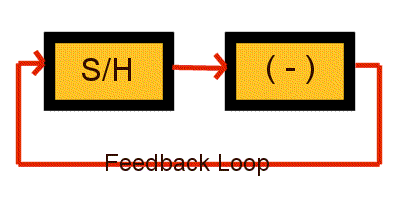
\includegraphics[width=90mm]{pics\lfo_feedback.png}
	\caption{Create a third LFO.}
	\label{third_lfo}
\end{figure}
S/H rate control input sets the overall frequency. Using the filter Modifier, you can get triangle waves. It can also be used for PWM, freeing up other LFOs for other uses!\\
Here are Two examples in Sysex format: \href{https://www.carbon111.com/sysex.zip}{two Examples}
The first one: ``ModifierLFO'' is a simple LFO example. Modifier 1 creates the squarewave and Modifier 3 smoothes the output of Modifier 1 (or 2).\\
The second one, ``Janmichelphaser'', is a simple solina string simulation with a phaser. Modifier 3 produces a triangle waveform using Modifier 1's square wave and modulates PW.
\subsection{Wavetable Browser}
A nice tutorial to create a patch that will allow you to fully audition each of the XT's wavetables. Actually rather handy! Submitted by vanHouten.\\

\section{Workshops}
% !TeX spellcheck = en_US
The workshops are collected from \href{https://www.carbon111.com/mwxt.html}{Carbon111}
\subsection{Vocal Sound Workshop Part 1}
A great tutorial by Snyxol(Alexander Eslava) graciously translated from the German by vanHouten (Fabian Logemann) and proofed and reworked by me. Originally published on \href{https://www.amazona.de/workshop-vocal-sounds-mit-dem-waldorf-microwave/}{Amazona.de}\\
``...how to make your MWII sing, moan or belch...''\\
\bigskip
Do you wish to create mystical, ghostlike or even angelic, wispy female to deep male ``oooooohhhhs'' and ``aaaaaahhhs'' like those popular in trance and ambient tracks? Consider yourself lucky to have an MW II/XT at your side as its a sublime tool to handle this - even better than a sampler. Its no surprise indeed, as you should bear in mind its an heir in the dynasty of the PPG-Wave-series, legendary for their synthetic choir sounds.\\

This article will explore several possibilities of synthesizing vocal-like sounds, from natural-human to alien-like and even metallic voices. Once in a while after you turn the knobs at random for a while, a more or less human sounding voice emanates from your machine. Every time this happens, you create (intentionally or not) the dominant formants like those of a human voice speaking a vowel. Formants are specific peaks in the frequency-spectrum that build up a kind of signature in the sound. For the synthesis of vowel sounds, only the loudest of the formants are relevant. If they were not expressed this way, people with different voices would hardly be able to understand each other because of the differences in their voice spectra. This vowel recognition paradigm paves the way for us to simulate vowels more easily. The vowel-formants are independent of pitch, which means while singing an ``aa-aa-aa-...'' melody, the ``aa''-related formants always remain at the same frequencies.
\paragraph{Using pure wavetables:}
	Let's start at the most obvious place:
	We will use wavetable \#64 (``Chorus 2''). This is kind of a pseudo multi-sample of a spoken "Aaaa" in 61 different pitches, such a collection of waves is necessary to make our ``Aaaa'' a realistic sounding vowel. If we played back a single wave using different pitches, its formant would be shifted as well, resulting in a mickey-mouse or monster-like voice. This wavetable was set up in the following way to counteract this:
	Make a Fourier-analysis of a deep male choir sample and derive a wave from the resulting spectrum using Fourier-synthesis (these waves sound like the original choir, but produces only a harmonic, thin and sterile tone). The other waves were made in the same manner, with their formants being shifted accordingly within the spectrum. For each note there is the correct wave, so each formant stays in tune. For an example, let's have a look at the patch ``Stenzels Chor''. This pad plays the right ``Aaa'' on each note, thus modulating Wave1 and Wave2. In this case it is useful to link Wave2-Startwave to Wave1-Startwave (using the Wave2-menu), to do that you only need to modulate Wave1, Wave2 will follow automatically.\\
	There are two ways of Modulating Wave1 :
	\begin{itemize}
		\item Wave1-menu: keytrack: +100\% (elegant)
		\item Mod Matrix: keytrack/keyfollow +56 -> Wave1 Pos (keyfollow also considers pitchbend and glide as well as tracking, thus its better)
		Reasonably, both Startwaves are set at 30 to cover the whole wave-range of 0-61; and don't forget to "limit" the wavetable (Wave1/2-menu) to avoid triggering the analog waveforms at the end of the each wavetable!
	\end{itemize}
Let's get to work and tune ``Stenzels Chor'' a little bit:
\paragraph{Fattening:}
First we should attempt to get a little more of a ``floating'' sound and make it more dense and blurred. The ``basic'' (Send-/Global-)Chorus is already working for us as it should be. Further detuning of the osc's might not be enough because it still sounds kind of weak and electronic. So, first we need to increase the number of voices:
\bigskip % Add an empty line
%These are optional parameters to finetune the placement of tables and figures, with the following meaning:
%
%h, here
%t, top
%b, bottom
%p, page of float
%e.g. \begin{figure}[!htb]
\begin{figure}[ht!]
	\centering
	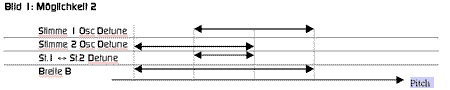
\includegraphics[width=90mm]{pics/vocal_workshop1_sol_2.gif}
	\caption{Fattening: Solution 2}
	\label{vocal_1_sol_2}
\end{figure}
\begin{enumerate}
	\item \emph{DualAssign}: Effectively we now have 4 oscillators and to make them sound more dense, we detune their pitches equally from each other (as is done with \emph{UnisonoAssign}): Consider the whole detune-width to be $n$ units. Our 4 pitches (4 osc's) have 3 gaps between them ->each gap is $n/3$ detune-units wide $\to$ The rule for equidistant detuning in \emph{DualAssign} with detune-width $n$:
	\begin{enumerate}
		\item First method: Osc1 Detune: $-n/6$; Osc2 Detune: $+n/6$; Trigger2 menu: Detune: $2/3\cdot n$
		\item Second method: Osc1 Detune: $-n/3$; Osc2 Detune: $+n/3$;	Trigger2 menu: Detune: $n/3$
	\end{enumerate}
	Let's choose the 2nd method with $n=45$. Set Osc1 Detune:-15; Trigger2 menu: Detune: 15\\
	More stereo? $\to$ De-Pan: 64...80. (Don't show off by De-Panning too much, because it thins out the floating sensation!). By engaging Pan-Delay for our purposes, the sound gets even thicker! Going from thick to thicker - there are two ways to get there; the first, \emph{Unisono Assign}, has the advantage of being extremely dense \& fat sounding - and you still have some effects to play with! The disadvantage is the loss of voices you might need for other purposes! The second method is to engage both chorus effects which may help you to get along quite well even with \emph{Normal Assign}, but you sacrifice the ability to use delay.
	\item \emph{UnisonoAssign}: Considering this method, one Osc should be sufficient, so turn down Wave2Level in the mixer first and enter
	Trigger2-menu: Detune: 40-55 ; De-Pan: 127\\
	By turning Wave2Level up again and detuning it slightly from Osc1, it becomes more dynamic and smoothly morphing: Osc1 Detune: -2; Osc2 Detune: +2\\
	Add some Pan-Delay and you should now have a really dense, deep choir. The beautiful ``floating'' is pleasant if the voice is triggered with short notes.
	\item Engaging both chorus effects: Even a monophonic, constant, sterile tone can be widened without increasing the number of voices by making use of the (Insert-)Chorus of the effects-section, combined with the (Send-)Chorus (the one without parameters). The latter one is fed by the output-sum of the first one (serial), thus you get effectively 8 delay voices added to the original voice. Well, it´s not really the same as with Unisono because the pitches of the echoes are shifting, but the result might be even warmer, more dynamic and wider in stereo separation than using \emph{Unisono Assign}. So don't be afraid to be a miser when it comes to effectively sparing voices.\\
	In our case we will work with \emph{Normal Assign}: Osc1Detune=-15; Osc2Detune: +15\\
	Set for Chorus: Speed: 65; Depth: 127, Mix: 0...127 $\to$ the more Speed, the more fat and wobbly it gets. Use values up to 68 for short notes, while slower pad-sounds go better with lower values about 53. In the case that lower frequencies have too much tremolo, decrease the mix-ratio or engage Filter2 as a HP.
\end{enumerate}
Controlling the position of the formants:
\begin{enumerate}
	\item Phase Shifting: For this purpose adjust Startwave 1/2 or the pitches. For playing around and testing purposes, it is reasonable to let only Wave1 through the mixer. Of course you can make use of the Modwheel to take control of Wave1. Wave2 will also follow as long as ``Link'' is set to ``On'' in the Wave2-menu. If you increase the Startwave positions, the formants will decrease and in doing so you might change the ``Aaa'' into an ``Ooo''. Have fun playing around using modulation-sources like the LFO or WaveEnvelope for formant shifting. This sounds like a kind of beautiful filter-sweep.
	\item No keytrack: As realistically ``vowel-like'' that wave modulation by Keytrack might sound, it is inflexible when it comes to playing melodies. It sounds just too bland, due to it's limitation to the vowel ``A'' - dull when its triggered by high notes, brighter when triggered by lower notes. When using analog waveforms such as sawtooth, of course all the formants are shifting along with the pitch. So set Wave1Keytrack to zero and adjust Pitch and Startwave accordingly to what kind of voice you want to hear, then play a melody which shouldn't exceed the range of two octaves.
	\item Appropriate Wavetables: 
	\begin{itemize}
		\item WT 028 (``FmntVocal'') is also a formant-sweep, quite narrow like a BP-filter and is useful to be "formant-shifted" by the WaveEnvelope. To get more bass into it, you might set both Startwaves to zero while tuning Wave1EnvAmount to a high value and Wave2EnvAmount to a lower one; Envelope times should be pretty slow to avoid harsh transitions.
		\item WT 057 (``MaleVoice'') consists of the vowels ``a,e,i,o,u''.
		\item WT 008 (``MellowSaw''), WT 009 (``Feedback'') and WT 010 (``AddHarm'') are also useful to create voice-patches.
		\item Combining certain different waves of WT 001 ("Resonant") or WT 025 (``ResoHarms'') some smooth and high voice-like sounds can be created as well. In this case Osc1 and Osc2 act as the formants.
		\item Even ultra-harsh waves like WT 044 (``FuzzWave'') might sound voicy, if they are dampened by the 24dB-LP and/or the Filter2-LP. 
	\end{itemize}
\end{enumerate}
\subsection{Vocal Sound Workshop Part 2}
Part two of Snyxol's great vocal tutorial, also translated by vanHouten. Originally published at \href{https://www.amazona.de/workshop-vocal-sounds-mit-dem-waldorf-microwave/}{Amazona.de}\\
"How to make your MWII/XT sing, moan or belch..."

Some sound patches described within this text are available for download at the bottom of this page.

\paragraph{ Pseudo comb-filter:}
...we pick up the track of part one at ``Alexander’s Choir'', but without the applied wavetable-modulation via keytrack. One can ``morph'' the formants of the wavetable by not detuning the oscillators. This way their phases will stay in a constant position and Osc2 will act as a very short delay of Osc1. Thus depending on the phase-shifting some of the upper harmonics are damped more than others or even vanish completely. This effect is similar to a positive comb-filter. The frequency-response of our low budget comb-filter will look like this:
\bigskip % Add an empty line
%These are optional parameters to finetune the placement of tables and figures, with the following meaning:
%
%h, here
%t, top
%b, bottom
%p, page of float
%e.g. \begin{figure}[!htb]
\begin{figure}[ht!]
	\centering
	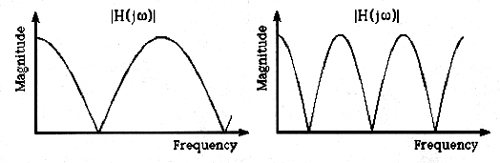
\includegraphics[width=90mm]{pics/comb_filter.png}
	\caption{Frequency over magnitude for the Comb-filter}
	\label{comb-filter}
\end{figure}
with $\omega = f \cdot 2 \pi = 2 \pi / T$. (Whereas $H$ is the transmission function, $\omega$ is the cycle-frequency. And $j = \sqrt{-1}$ is a constant value derived from the complex numbers $j \in \mathbb{C}$.) But don’t be intimidated by the mathematics, because that’s not the reason why we're here. As can be seen in the plot, there are equidistant gaps notched into the spectrum, which get narrower according to the amount of delay. The spectrum gets "combed", creating new formants.\\
Let’s go to work then, fixing the phase-length of the oscillators. By activating "sync", we would force the phase-shift to zero.....so we avoid doing this!!
If the arpeggiatior is active, switch on poly-mode as well! The reason is that the arpeggiator or even playing legato in mono mode and normal/dual assign lets the oscillators run freely and thus out of phase. This would hinder us from starting the phases with the note-on-event. To keep the sound fat enough, we choose dual assign \& Detune: 15-30 while engaging both chorus effects, just like we did last time.\\
$\to$ Osc1+2 Detune:0; Mixer-Wave 1+2: 63; Wave1: Phase: 3°\\
...then playing around with the phase of wave2, we can hear the change in the sound as it is altered by our ``low-budget-comb''. 
\begin{example}
	If Wave2 Phase = 183°, then all odd harmonics are swept away.
\end{example}

\paragraph{RM, Waveshaping:}
Let us start here with a few examples
\begin{example}
	\begin{enumerate}
		\item ``HyperSweetVox1'': Use WT \#012 (``WindSyn'') and choose Wave \# 000.\\
		This wave sounds oboe-like, hardly a voice. We can change that by ringmodulating it with a square-wave:
		
		Wave2: square
		Mixer: ringmod=127, all others zero
		
		Set the tuning of the two oscillators to an equal value. Detuning of the oscs would create strange, rough distortion. The ringmodulated signal only sounds smooth and voicelike with a square, if the oscillators are humming in certain phases:
		
		Wave1/2: startphase= 003°
		Wave2: startphase= 93°
		
		For fattening the sound, one can use UnisonoAssign or use the methods of the first part of this workshop.
		For a filter, let’s use the Sin(x)->LP: CutOff= 127 , so nothing will be filtered at all but distorted instead. The Sinus-shaper is a kind of an overdrive which is positioned after the mixer and before the 12dB-LP-filter; If the mixer-output-signal stays beneath 64 (half the maximum), the shaper provides a smooth saturation; as the mixer-signal increases beyond this threshold, the wave peaks will no longer be flattened, but inverted: e.g. a sawtooth-wave will be morphed to a sine-wave. The spectrum of this distorted signal depends mainly on the input-signal-level.
		
		
		The higher thte ringmod-amount, the more "smokey" and "wooden" the sound of the voice. At lower levels (<63) the distortion is hard to recognize, but is a usefull little gimmick for recording as the volume of the sound is increased, unlike with the 24dB-filters.
		You can modulate the ringmod amount through key-velocity for example:
		
		Mixer: Ringmod= 36
		ModMatrix: Mod1: velocityàRingmod  amount=+63
		
		Feel free to use e.g. a triangle for wave2 and sweep through the startphases. Rising from 3° to 93° the result reaches from muffled to bright and misty.
		\item ``ResoVox1'': we have the values:
		\begin{itemize}
			\item Trigger2menu: mode=poly
			\item Assign= dual
			\item Detune=15
			\item De-Pan=86
			\item (Send-)Chorus= on
			\item FX: Pan-Delay= 1/8 [80]; 53; 90:37
			\item WT: 25 (ResoHarms)
			\item Wave1: Startwave=30
			\item Wave2: Startwave=30
		\end{itemize}
		We will sweep through the startwave-positions via the Lfo’s with a triangle shape. For more agility, let the LFO-phases of the two voices (DualAssign) drift out of sync with each other. Which means e.g. LFO1 to be assigned to two different phases within the both voices. And due to the voices being spread with stereo-panning, wave1 will play a different wave on the right speaker than it does on the left side.
		To get this effect, LFO1/2Sync has to be switched off while Humanize= ~40.
		
		ModMatrix:  LFO1 -> Wave1Pos; amount=+55
		LFO2 -> Wave2Pos; amount=+55
		LFO1: Speed=29; startphase=3°
		LFO2: Speed=40; startphase=107° (as you wish, try...)
		Tuning: both oscs equal, all parameters set to zero
		
		Filter1: 24/12dB-LP or even no filtering activity at all
		Filter2: HP; +55; +50\%...to dampen the heavy bass-section.
		
		...use the ModWheel as a cross fader to shift between RingMod and Wave1+2:
		
		Mixer:  Wave1/2: 63; RingMod: zero
		
		ModMatrix: ModWheel $\to$ RM; Amount: +63
		ModWheel $\to$ Wave1Mix; Amount: -56
		ModWheel $\to$ Wave2Mix; Amount: -56
		
		that's all for now, folks!
		Have a nice day and `till next time
		Examples for download: http://www.amazona.de/waldorf/Vocal.zip \footnote{The Preset is sadly gone.}
	\end{enumerate}
\end{example}
\subsection{Waveshaping Workshop Part 1}
\notes{There is not 2nd part? Never released - sad.}
Part one of Snyxol's very in-depth waveshaping workshop. An invaluable look into one of the most powerfull sound-shaping aspects of the µWaveII/XT! This section is heavy on theory and the math behind waveshaping. (Part 2 will cover application and programming). Originally published at \href{https://www.amazona.de/workshop-waveshaping-mit-dem-waldorf-microwave/}{Amazona.de}\\
Waveshaping can be described as an extension of overdrive, which can be used to alter a sound from subtle to extreme using only a few parameters. This synthesis method provides sounds ranging from "distorted through the roof" to smooth, fluid or even more complex soundscapes. The most flexible shaper within the µWave 2/XT/XTk/pc is the waveshaper-filter. Closely related to this is the Sin>LP-filter. The mixer before the filter in the signal path is capable of distorting the audio-signal in a couple of ways also. Furthermore the µWave provides us with an overdrive in the effects section.

Although it is up to each sound craftsman to create his sounds by continually trying, trying, trying.... there are certain cases, in which the slightest alteration of parameters may lead to radical results and the waveshaper-filter is such a case. Thus being familiar with the behaviour of a waveshaper is essential while attempting to create particular kinds of sounds. So let's begin with the basics of waveshaping-synthesis and see what "mutilations" the shapers in the µWave can do to the waves.

This will require some math, but don't be intimidated! It´s almost all high-school level!!

We will address detailed sound programming tips in the next workshop due to the size of this particular topic.

1) What is wave-shaping?!
A shaper is a function $f(x)$, which depends on only one variable $x[n]$. $x[n]$ is the $n$-th sample of a control or audio signal. Thus $n$ is equivalent to the time, which in digital systems is quantized by the sampling-rate.

Alternatively one can imagine a shaper as a table, which maps every input value $x$ to an output value $y=f(x)$.

Trivial special case: the \emph{linear function} $f(x)=a\cdot x$ with the constant a is an amplifier. It simply increases or decreases the volume of the signal without changing the sound itself. Only the non-linear functions deserve the title ``shaper''.

linear: a function is linear exclusively while: 
\begin{enumerate}
	\item $f(a\cdot x) = a \cdot f(x) \with a=\const$
	\item $f(x+y) = f(x)+f(y)$
	\item Can be combined to $f(a\cdot x+b \cdot y)=a \cdot f(x)+b \Cdot f(y) \with a,b=\const$
\end{enumerate}
Non-linear functions applied on audio-signals result in a distortion of the wave, which changes it's spectrum in a very weird and very difficult to describe way. Some overtones may be added or amplified while others are dampend, like in a very complex filter. So may we speak of a shaper as a filter?! Nope!

Differences between a filter and a shaper:
Filter: only the spectrum of the input wave is relevant. The waveform has no direct influence on the sound color of the filter output. The phases of the harmonics might be deliberately shifted (which changes the waveform, not the sound). It changes the spectrum distinctly (side-effect: the waveform changes, of course).

Furthermore it is just linear*. Which means:

1. if the input-amplitude is changed by the factor a, then only the output-amplitude is changed by a, as well. The spectrum however remains the same.
2. It doesn't matter, whether two waves are first mixed and then filtered, or vice versa. One can't hear whether a sound contains one voice, in which two detuned sawtooth of equal amplitude are filtered, or two detuned voices in each of which only one sawtooth is filtered.

Waveshaper: only the waveform of the input wave is relevant. The spectrum of the input-wave has no direct influence on the sound color of the waveshaper output. Thus the phases of the harmonics must not be shifted freely, because this would bend the waveform itself and changing the tonal color. It distorts the waveform distinctly which is followed by a complex change of the spectrum most of the time.

In general a shaper-function is non-linear:
\begin{enumerate}
	\item if the input-amplitude is changed, then also the waveform and thus the spectrum.\\
	There is an exception: $f(x)=x^2$; $f(a \cdot x) = a^2 \cdot x^2$. the wave $x^2$ only changes it's amplitude while the form and the spectrum remain constant; this is generally valid for exponential functions
	\item it is a relevant difference whether two waves are first added or distorted. If the sum of two equal, detuned oscs is distorted, the result will be a periodic, wobbling changing of the sound, which may sound more or less earthy and strange, depending on the shaper-function. If a normal detune-hovering is required (as without distortion), there are two detuned voices to be used per note and one shaped osc per voice (or even both shaped, but not detuned).
	
	While FM distorts a wave horizontally (in time), wave-shaping distorts it vertically.
	
	If a shaper is placed immediately after an oscillator, the result is a new constant waveform with a new harmonic spectrum which can be deliberately filtered.
	
	Even more fascinating is shaping placed after the filter. The most well-known type is probably the filter-overdrive, which enriches a muffled low-pass-filtered sound with new, even different harmonics and thus modifies it from warm and dark to crunchy and rough. This post-filter-distortion destroyes the prior work done by the LP-filter (dampening higher harmonics). The filter is mainly abused for changing the waveform of the oscillator. Eventhough a filter-sweep sounds very smooth and the spectrum morphs slowly, the filter modifies the output-wave quite heavily, even with slow cutoff frequency modulation and mainly at great resonance-values.
	
	Since, as is well known, the shaper reacts on waveform-changes, the shaper-output morphs stunningly fast. The result is a wild, crazy and drastically changing sound.
	
	Though there is snag: Aliasing. Even if the oscillator is band-limited (free of aliasing), the shaper function adds frequencies to the spectrum which are above half the sampling rate (NYQUIST-frequency). Digital audio systems cannot handle those above-Nyquist-frequencies correctly, but mirrors their frequencies around half the sampling rate, which transforms those overtones into wrong ones (``alias'' tones), sounding dissonant and metallic-like. This is not necessarily awful-sounding , it´s a matter of taste and sound category. E.g., aliasing can add a cool digital spice to aggressive distortion sounds.
\end{enumerate}

\begin{example}
	then some example for the function $f$ to generate some nice waveshaping:
	\begin{enumerate}
		\item Parabolic distortion via $f(x)=x^2$: All input-samples are squared. A sawtooth-wave e.g. is distorted to an overtone-poorer parabolic wave. (this can also be accomplished by Ringmodulation: multiply two sawtooth-waves of equal phases)
		\bigskip % Add an empty line
		%These are optional parameters to finetune the placement of tables and figures, with the following meaning:
		%
		%h, here
		%t, top
		%b, bottom
		%p, page of float
		%e.g. \begin{figure}[!htb]
		\begin{figure}[ht!]
			\centering
			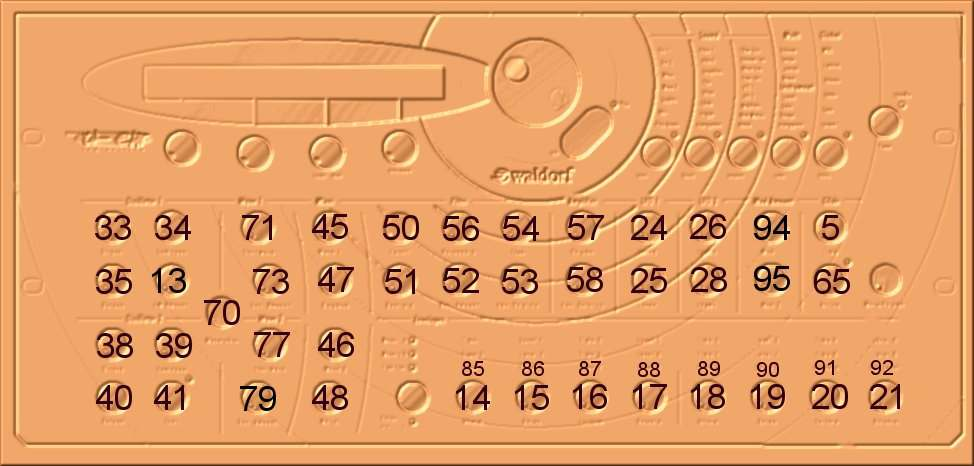
\includegraphics[width=90mm]{pics/xt_midi_chart.jpg}
			\caption{MIDI CC numbers and their associated knobs}
			\label{midi_cc_interface}
		\end{figure}
		\bigskip % Add an empty line
		%These are optional parameters to finetune the placement of tables and figures, with the following meaning:
		%
		%h, here
		%t, top
		%b, bottom
		%p, page of float
		%e.g. \begin{figure}[!htb]
		\begin{figure}[ht!]
			\centering
			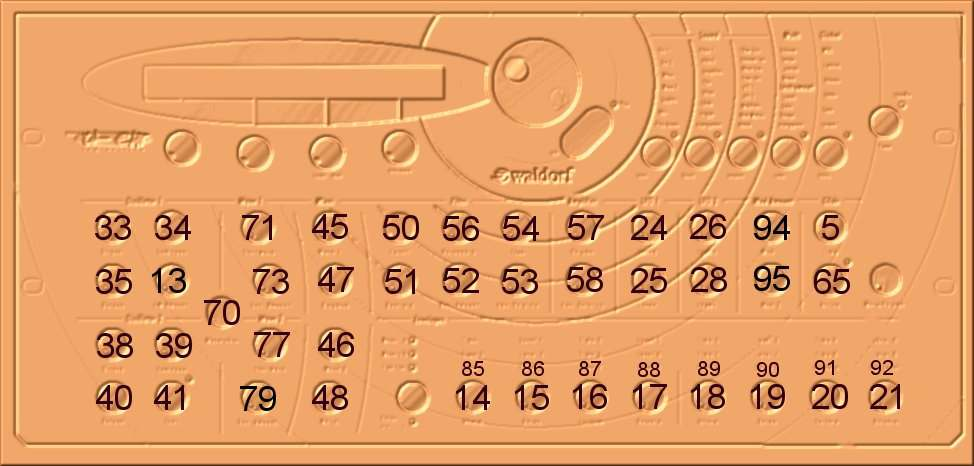
\includegraphics[width=90mm]{pics/xt_midi_chart.jpg}
			\caption{MIDI CC numbers and their associated knobs}
			\label{midi_cc_interface}
		\end{figure}
		\bigskip % Add an empty line
		%These are optional parameters to finetune the placement of tables and figures, with the following meaning:
		%
		%h, here
		%t, top
		%b, bottom
		%p, page of float
		%e.g. \begin{figure}[!htb]
		\begin{figure}[ht!]
			\centering
			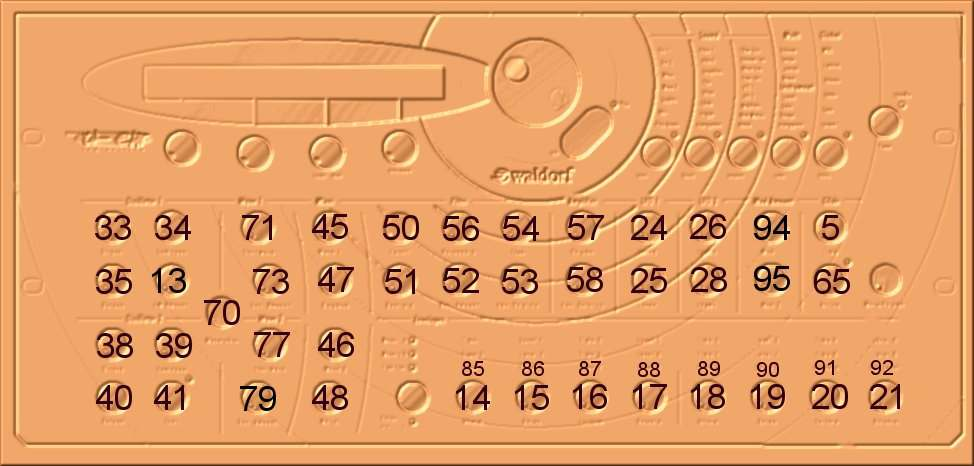
\includegraphics[width=90mm]{pics/xt_midi_chart.jpg}
			\caption{MIDI CC numbers and their associated knobs}
			\label{midi_cc_interface}
		\end{figure}
		\item Exponentiator via $f(x)=a \cdot exp(b\cdot x)$ with constants $a,b$: ...is often used for controller-signals. Using this a synthesizer computes the frequency of its oscillator deriving from the note-number. In general all logarithmically scaled parameters like volume, LFO-Rate and envelope-times are transformed this way.
		\item Hard-clipping via $f(x)= {x, for |x|<1}$ with the absolute value, which splits into two sets: ${+1, for x>+1}$ and
		${-1, for x<-1}$
	\end{enumerate}
\end{example}
c) 

The signal x gets abruptly limited to the range of [-1;+1]. Dull waves are enriched with many harmonics. While using as filter-overdrive, the result sounds harsh scratching, works great for biting agressive sounds.



d) Soft-clipping / saturation: e.g. f(x)=(arctan x)/pi
or
f(x)=(sign x) *(1-0,25/(|x|+0,25)) (build up of hyperbolics)
or
f(x)=1-(x-1)² , for 0<=x<1; |
f(x)=-1+(x+1)² , for -1 f(x)=sign x , for |x|>=1 |

The signal x is smoothly limited to the range of [-1;+1]. Contrary to hard-clipping, the signal is not cut abruptly, but follows the smooth transition to the saturation value. This enriches dull sounds with more low and middle than with high harmonics. There are many possible functions for this same effect, but they all sound different.

Analog tapes creates a similar saturation-behaviour which provides a mix with a warm characteritic. (Because of this behviour many producers prefer to work with old tape decks rather than using digital epuipment.)

This effect is also suitable for filter-overdrive: decreasing amplification before saturation results in a warm, smooth grunge. Using extremely high pre-amplification ends up with a harshness equal to hard-clipping.



2)Mixer-Clipping: Overflow and Saturation
as described on page 46 in the manual.

The mixer of the oscillator section applies it´s own waveshaper (with 2 selectable functions) on the sum of the input signals (ringmod + noise + wave1 + wave2), limiting the output to the range [-M;+M], with:

M: maximal mixer output amplitude

(though the ROM and RAM waves are stored in only 8 bit resolution (quantizing to 256 steps), the output of each oscillator is a smooth interpolated 24 bit depth signal. the Motorola 56303 DSP inside the MW2 computes with 24 bit fixpoint numbers, providing 16.7 million equally big quantization steps.)

The "saturation" mode does hardclipping.

"Overflow" distortion mode: to samples of the mixer sum, which are in the forbidden range of x>+M OR x<-M, the values -2M or +2M, respectively, are added. This simulates the numeric overflow of the µ-Wave1 and PPG Wave. The harsh transitions generated by the overflow-clipping are equivalent to adding pulse-waves (with variable pulse width).
Another way to visualize overflow:
if the level of the mixer-sum is beyond legal range, some "magic" pulse-waves are mixed into it (see graphics). Those pulse wides can be well-directed adjusted by modulating the amplitudes of the mixer-input-sources.

Overflow function: f(x)= {x, for |x|<=M}
{x-2M, for +M {x+2M, for -3M<=x<-M}
	
	(this formula is applicable only if wave1+2 and ringmod are chosen in the mixer. This way the sum never exceeds 3M. If noise or the external input is engaged as well, any sum-sample may overflow even two times.)
	
	
	
	...always beware of overflow introducing heavy aliasing.
	
	3) Sin(x)->LP-Filter
	Here is a sine-shaper inserted after the mixer and BEFORE a 12dB-LP-filter. Because the mixer-output is always within the values of [-M ; +M], the definition range (possible x values) [-M ; +M] is sufficient for the shaping function. At increasing amplitude the input-signal first gets compressed softly at the upper and lower peaks. As the amplitude exceeds the M/2-threshold, peaks get wrapped towards the zero axis.
	
	Sinus-Shaper: f(x) = M * sin (p /M * x), -M <= x <= +M
	
	
	
	
	
	example: 2 waves of increasing amplitude becoming more and more squeezed:
	
	
	
	
	
	
	
	By combining Sin->LP-filter and overflow-mixer-ditortion, the overflow-jumps will be eliminated totally because the signal values -M and +M are bent to zero. The resulting distortion can sound even smoother than engaging saturation type mixer-clipping.
	
	4) Waveshaper Filter
	First of all and contrary to the Sin(x)->LP-filter, the Shaper is routed AFTER the 12dB-LP-filter. This routing provides grungy filter-overdrive and much more crazier sounds. Further one can choose an arbitrary wave out of the current wavetable to define the shaping function. I refer to this wave as "shaper-wave". (don´t mess it up with the wave that GETS shaped!) It is exactly this feature that makes the waveshaper a very flexible distorter, gifted far beyond common hard/soft overdrive like that found in many other analog/ v.a. synthesizers.
	
	Fast filter-sweeps at high resonance create hard, weird, dirty and often screaming distortion. (reasons: see section 1)
	
	Softer and less agressive sweeps are achievable by very, very slow filter-sweeps and low cutoff, or even without any filtering while slowly modulating only one´s or both´s oscillator's amplitudes (not detuned) in the mixer.
	
	Now what does the distortion-function f(x) look like, that is defined by a particular shaper-wave?
	
	Briefly: its the same as the shaper-wave itself from 90° to 270° (samples 32...97), but interpolated linearly.
	
	Specifically: the output level of the filter itself is limited to 2M (twice the mixer-output), no matter how high the resonance is cranked up. Thus the definition range (allowed input values) of the shaper-function has to be [-2M ; +2M]. Output-values produced by the shaper roam within these borders as well.
	
	A wave-cycle is always made of 128 samples. Mostly the wave reveals an odd symmetry: the first half is fetched from ROM/RAM, the second is it's mirror-image on the point (64,5 ; 0). Formally:
	
	Wave[65 + n] = -Wave[64 - n], n = 0, ..., 63
	
	Among the ROM-wavetables in the µWave2/XT/XTk, WT 65 "True PWM" (which emulates the normal pulse-oscillator) is the only one without this type of symmetry.
	
	In the shaper-wave, only samples 32 to 97 are relevant; the first and latter 31 samples are without any effect. Neighbouring shaper-samples are interpolated linearly, giving the function the shape of a continous polygon. Accordingly there are no jumps in it, only steep transitions are possible.
	
	The definition range [-2M ; +2M] refers to the sample-range [32,5 ; 96,5].
	
	E.g: Input-value "-2M" is mapped to the average of samples 32 and 33:
	f(-2M) = (Wave[32] + Wave[33]) / 2;
	f(+2M) = (Wave[96] + Wave[97]) / 2;
	
	The plot of this function equals the wave-cycle from 90° to 270° (samples 32...97), except that neighbouring samples are connected by a straight line instead of a smooth, round interpolation curve. In the picture "shaper-wave" below the pink frame contains a plot of the corresponding shaping function.
	
	
	
	
	... now let's engage this function to shape a triangle-wave of rising amplitude (without filtering):
	
	
	
	
	
	
	
	Preservation of Odd Harmonics
	All shaper waves, except from WT "True PWM", generate shaping functions pointsymmetric to the origin (odd symmetry):
	
	(1) f(-x) = - f(x)
	
	A big advantage of such a shaper is that the output wave has odd harmonics only, if the input wave consists only of odd harmonics, too. At deep pitches shaped filter sweeps with odd harmonics only sound hollow and mostly more pleasant (for my taste), whereas waveshaped sounds with both even and odd harmonics (like saw) have a more dirty and woody character. But on high pitches, odd harmonics sound more flute-like, and sounds with both even and odd harmonics could be nicer. (that´s only my personal feeling, but I want to give a guideline for waveshaping sound programming beginners ;-))
	
	Now I want to prove the property:
	(2) odd symmetric shaper functions preserve odd harmonics.
	
	!!! big math-haters can skip the rest of this article!!! :)
	
	x(t) is a audio signal depending on time. If this signal is a periodic waveform, then T is it´s cycle lengh.
	(periodic means: x(t+k*T)=x(t), for k=...,-1,0,1,2,...)
	
	(3) A wave consisting of odd harmonics is equivalent to the symmetry:
	x(t+T/2) = - x(t)
	(visually: the 2. half is the sign inverted copy 1. half)
	
	Proof for (3):
	
	´=>´: a sine wave with a frequency that is an odd multiple of the base frequency has this symmetry. And a sum of two such odd overtones has this symmetry, too:
	y(t): sum wave
	x1(t), x2(t): sinoids
	y(t+T/2) = x1(t+T/2)+x2(t+T/2) = -x1(t)-x2(t) = -y(t)
	
	´<=´: Consider a wave x(t) with the symmetry x(t+T/2) = - x(t). Dismantle it into a sum of a wave xO(t) containing it´s odd harmonics and a wave xE(t) consisting of it´s even overtones:
	(6) x(t)=xE(t)+xO(t)
	a sine wave x1(t) with a frequency that is an even multiple of the base frequency has the symmetry:
	x1(t+T/2) = + x1(t)
	
	In a little proof analog to the above ´=>´ proof, one can show that the sum of two even harmonics has the same symmetry, too. This implicites:
	(4) xE(t+T/2) = + xE(t)
	Whereas the odd part has the property:
	(5) xO(t+T/2) = - xO(t)
	first (6) and then (4) and (5) into (3):
	x(t+T/2) = - x(t)
	xE(t+T/2)+xO(t+T/2) = -xE(t)-xO(t)
	xE(t)-xO(t) = -xE(t)-xO(t)
	
	* xE(t)=0
	Means : no even harmonics.
	
	Proof for (2):
	We insert an odd harmonic wave into an odd symmetric shaper function.
	y(t) is the output wave, x(t) the input.
	To show: y(t+T/2) = - y(t)
	Using (1) and (3):
	y(t+T/2) = f(x(t+T/2)) = f(-x(t)) = -f(x(t)) = -y(t)
	Snyxol
	Snyxol@web.de
	
	A slightly different version of this workshop was originally published at Amazona.de
\subsection{Sound On Sound's MWXT Masterclass}
An excellent resource and in-depth tutorial of our favorite orange synth from the Jan '03 issue of the best music gear magazine out there! One minor caveat though - the author obviously dosen't know about the "limit" function in the wavetable menu.\href{https://www.soundonsound.com/techniques/getting-creative-waldorf-microwave-synths}{SOS January 2003}\\
\section{Information about the wavetables}
% !TeX spellcheck = en_US
This is the description of the PPG Wave 2.2 wavetables as used in the Microwave II/XT. (Plus Wavetable 64).
\begin{itemize}
	\item 001 Resonant: Harmonics 1-8 very strong, simulation of a resonant filter,wave number 00 is a sine wave.
	\item 002 Resonant 2: Similar to wavetable 00, but with additional higher harmonics, dual VCF simulation.
	\item 003 MalletSyn: Similar to two previous wavetables, but also good for vibes, bells, tubular bells, and so on.
	\item 004 Sqr-Sweep: Sine-to-rectangular sweep, low-resonance VCF simulation, clarinette and flute sounds
	\item 005 Bellish: Waves 00-47 feature very high harmonics in progressively greater amplitudes. Waves 47-59 continue to add high harmonics but at a faster rate. Also useful for delay effects and church bells.
	\item 006 Pul-Sweep: Very high harmonics are emphasized, effects similar to wavetable 15, but more mixture-like.
	\item 007 Saw-Sweep: Sine-to-ramp sweep, low-resonance-VCF effects, also good for woodwinds.
	\item 008 MellowSaw: VCF sweep without resonance, also useful for woodwind sounds.
	\item 009 Feedback: Highpass VCF simulation without resonance. Wave 00 has little or no fundamental. Wave 25 has fundamental at maximum amplitude. Useful for dark percussive strings, bass with click-like attack.
	\item 010 Add Harm: Formants are strong middle-range harmonics, useful for ring-modulation and vocal sounds
	\item 011 Reso 3 HP: Similar to wavetable 09.
	\item 012 Wind Syn: Low formants. Wave 00 is dark, 32 is bright, 59 is dark.
	\item 013 High Harm: High formants that sweep.
	\item 014 Clipper: Very strong high-order harmonics, the fundamental is weak. Useful for bright percussive stringed keyboard instrument sounds like clavichord, harpsichord, and so on. When swept, you get an amplitude modulation effect. Wave 00 is maximum amplitude, 24 is minimum amplitude, 59 is maximum. Use great detuning, upper waves and dissonant low chords for noise effects.
	\item 015 Organ Syn: Several organ registers. Sine, Hammond, Lowery, Church organs.
	\item 016 SquareSaw: Harmonics 2 + 3 to sawtooth sweep. Useful for harmonium, accordian, harmonica sounds.
	\item 017 Formant 1: Wild amplitude modulation effects when swept. Several peaks and dips in amplitude.
	\item 018 Polated: Wave 00 features the fundamental and second harmonic. Wave 14 is the fundamental alone. Wave 40 has high harmonics. Wave 59 is the fundamental alone.
	\item 019 Transient: When swept produces high-low-high harmonic sweep effect.
	\item 020 ElectricP: Waves 00-32 are stationary waveforms with string upper harmonics and a few lower harmonics. Wave 59 has no fundamental.
	\item 021 Robotic: Fast discrete changes of low and high harmonics for sample and hold effects. Wave 00 is a sine wave.
	\item 022 StrongHrm: Sine wave to high frequency formants.
	\item 023 PercOrgan: This wavetable is particularly suited for echoing effects. Waveforms vary from original attack plus one delay, to two colored delays. Wave 00 is a sine wave.
	\item 024 ClipSweep: Strong high harmonics.
	\item 025 ResoHarms: Stationary organs. If swept produces ascending high harmonic sweeps.
	\item 026 2 Echoes:	Waves 59 to 49 go from bright to sine wave. 48 to 33 have a colored delay. 33 to 18 are sinewaves. 17 to 00 have a colored delay echo.
	\item 027 Formant 2: Variations on sawtooth waves is strong, bright formants. Good for brass sounds.
	\item 028 FmntVocal: Formant sweeps. When keyboard is used to control the waves vocal and choir sounds can be produced.
	\item 029 MicroSync: Phasing sawtooth waves. Useful for ensemble string sounds.
	\item 030 Micro PWM: Square to rectangular to narrow pulse waves. Sweeps produce pulse-width modulation effects.
	\item 064 Chorus 2: Description by Wolfram Franke (Dec. 1999): "The wavetable is an analysis of a
	male choir sample I did 5 years ago for the Wave. The original choir pitch
	was F 1 and the Wave transformed it so that it generates an equal formant
	spectrum through the whole keyboard range."
\end{itemize}
What about the other ones?
\section{MIDI stuff}
% !TeX spellcheck = en_US
\subsection{Microwave XT Continuous Controllers Chart}
Paul Nagle has graciously granted permission to provide this handy reference chart of MIDI CC numbers and their associated knobs. Great if you want to use the Microwave XT's control surface to manipulate other synths and/or software.\\
\bigskip % Add an empty line
%These are optional parameters to finetune the placement of tables and figures, with the following meaning:
%
%h, here
%t, top
%b, bottom
%p, page of float
%e.g. \begin{figure}[!htb]
\begin{figure}[ht!]
	\centering
	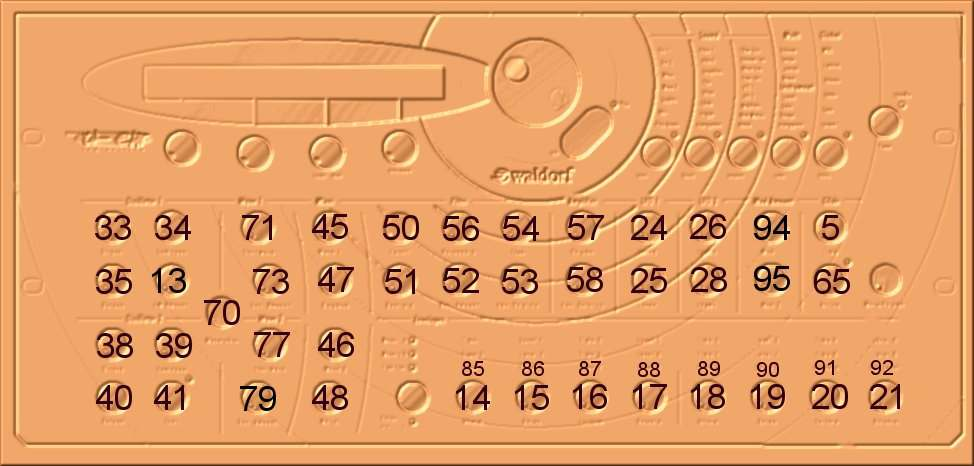
\includegraphics[width=90mm]{pics\xt_midi_chart.jpg}
	\caption{MIDI CC numbers and their associated knobs}
	\label{midi_cc_interface}
\end{figure}
\section{Additional reading material/References}
% !TeX spellcheck = en_US
%\clearpage
\todo{Not working!}
\bibliography{mwxt} 
%\bibliographystyle{apalike}
\bibliographystyle{alpha}
\end{document}
